\documentclass{article}
\usepackage{template}

\usepackage{chngcntr} % Reset counter within sections
\usepackage{circuitikz}

\counterwithin*{equation}{section}
\counterwithin*{equation}{subsection}

\pagestyle{fancy}
\setlength\headheight{24pt}

\lhead{\className}
\rhead{\leftmark}
\cfoot{\thepage}

\newcommand{\uniTitle}{Queensland University of Technology}
\newcommand{\className}{Foundations of Electrical Engineering}
\newcommand{\classTime}{Semester 2, 2021}
\newcommand{\classInstructorName}{Dr Sam Cunningham-Nelson}
\newcommand{\authorName}{Tarang Janawalkar}
\newcommand{\authorStudentNumber}{n11032201}
\newcommand{\classCode}{EGB120}

\usepackage[
    type={CC},
    modifier={by-nc-sa},
    version={4.0},
    imagewidth={5em},
]{doclicense}

\date{}

\begin{document}
\begin{titlepage}
    \vspace*{\fill}
	\begin{center}
        \LARGE
        \textbf{\className}
        \texorpdfstring{\\}{ }
        \uniTitle
        \texorpdfstring{\\}{ }
        \texorpdfstring{\vspace{0.3in}}{ }
        \normalsize\textit{\classInstructorName}
        \texorpdfstring{\\}{ }
        \classTime
    \end{center}
    \begin{center}
        \textbf{\authorName}
    \end{center}
    \vspace*{\fill}
    \doclicenseThis
    \thispagestyle{empty}
\end{titlepage}
\newpage

\tableofcontents
\newpage

\section{Electrical Circuits}
\subsection{Fundamental Quantities}
\begingroup
\renewcommand{\arraystretch}{1.5}
\begin{table}[H]
    \centering
    \begin{tabular}{c | >{\centering}p{0.5\textwidth} | c c}
        \toprule
        \textbf{Name} & \textbf{Definition} & \textbf{Symbol} & \textbf{Unit} \\
        \midrule
        Charge & Electric charge is a fundamental property of matter that governs how particles are affected by an electromagnetic field.
        & $q$ & Coloumb (\unit{\coulomb}) \\
        \hline
        Current & $i=\dv{q}{t}\iff\SI{1}{\ampere}=\SI{1}{\coulomb\per\s}$
        & $i$ & Ampere (\unit{\ampere}) \\
        \hline
        Voltage & $v=\dv{w}{q}\iff\SI{1}{\volt}=\SI{1}{\joule\per\coulomb}$
        & $v$ & Volt (\unit{\volt}) \\
        \hline
        Power & $p=\dv{w}{t}\iff\SI{1}{\watt}=\SI{1}{\joule\per\s}$
        & $p$ & Watt (\unit{\watt}) \\
        \bottomrule
    \end{tabular}
\end{table}
\endgroup
\begin{description}
    \item[Charge in an electron.] $q=\SI{1.6022e-19}{\coulomb}$.
    \item[Electric Power.] $p=\dv{w}{t}=\frac{\dd{w}}{\cancel{\dd{q}}} \frac{\cancel{\dd{q}}}{\dd{t}}=vi$. 
\end{description}
\subsection{Passive Sign Convention}
\begin{figure}[H]
    \centering
    \begin{minipage}[H]{0.48\textwidth}
        \textbf{Passive component}
        \centering
        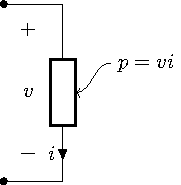
\includegraphics[height = 4cm, keepaspectratio = true]{passive_component}
        \caption{Energy dissipated.}
    \end{minipage}\hfill
    \begin{minipage}[H]{0.48\textwidth}
        \textbf{Active component}
        \centering
        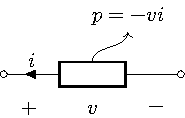
\includegraphics[height = 4cm, keepaspectratio = true]{active_component}
        \caption{Energy produced.}
    \end{minipage}
\end{figure}
\begin{theorem}[Power Balance]
    \begin{equation*}
        p_{\mathrm{net}} = 0
    \end{equation*}
\end{theorem}
\begin{theorem}[Energy]
    \begin{equation*}
        w\left( \tau \right) = \int_0^\tau p\left( t \right) \dd{t}
    \end{equation*}
\end{theorem}
\subsection{Circuits and Sources}
\begin{definition}[Circuits]
    A circuit is a mathematical model that approximates a real system. It is built from ideal circuit elements connected by ideal wires. 
\end{definition}
\begin{definition}[Voltage Source]
    Produces or dissipates power at a specified voltage with whatever current is required. 
\end{definition}
\begin{figure}[H]
    \centering
    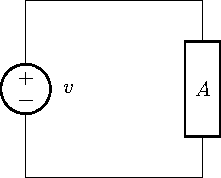
\includegraphics{voltage_source}
    \caption{Voltage Source -- $v$ is specified, $i$ varies depending on circuit element $A$.}
\end{figure}
\begin{definition}[Current Source]
    Produces or dissipates power at a specified current with whatever voltage is required. 
\end{definition}
\begin{figure}[H]
    \centering
    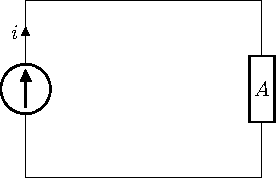
\includegraphics{current_source}
    \caption{Current Source -- $i$ is specified, $v$ varies depending on circuit element $A$.}
\end{figure}
\subsection{Ground}
\begin{description}
    \item[Definition.] The zero volt point is referreed to as the circuit ground.
    \item[Symbol.] \tikz\draw (0, 0) node [sground] {};
\end{description}
\subsection{Earth}
\begin{description}
    \item[Definition.] An earthed ground is literally a connection to the earth.
    \item[Symbol.] \tikz\draw (0, 0) node [ground] {};
\end{description}
\subsection{Connected Sources}
\begin{figure}[H]
    \centering
    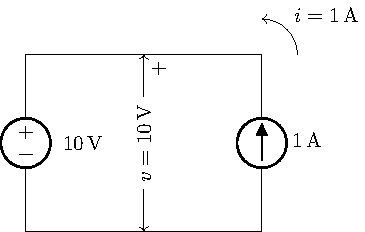
\includegraphics[height = 4cm, keepaspectratio = true]{connected_sources}
    \caption{Example of a connected voltage and current source.}
\end{figure}
\begin{itemize}
    \item The voltage source sets $v$ to \SI{10}{\volt}, with the upper wire being positive.
    \item The current source sets $i$ to \SI{1}{\ampere}, flowing anticlockwise.
    \item Therefore \SI{10}{\watt} of power is produced by the current source and dissipated by the voltage source.
\end{itemize}
\begin{enumerate}
    \item Two voltage sources must be connected at the same terminals and supply the same voltage.
    \item Two current sources must flow in the same direction and supply the same current.
\end{enumerate}
\subsection{Invalid Circuits}
\begin{figure}[H]
    \centering
    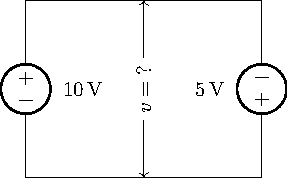
\includegraphics[height = 4cm, keepaspectratio = true]{invalid_voltage_sources}
    \caption{Voltage terminals are incorrect, and voltages are different.}
\end{figure}
\begin{figure}[H]
    \centering
    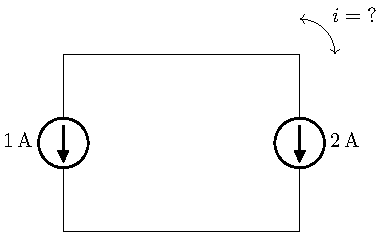
\includegraphics[height = 4cm, keepaspectratio = true]{invalid_current_sources}
    \caption{Current flows oppose each other, and currents are different.}
\end{figure}
\subsection{Resistors}
\begin{definition}[Resistor]
    Dissipates power so that the voltage across both terminals is proportional to the current.
\end{definition}
\begin{figure}[H]
    \centering
    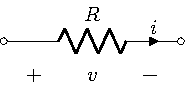
\includegraphics[height = 4cm, keepaspectratio = true]{resistor}
    \caption{}
\end{figure}
$v=iR$
$r=\frac{\rho L}{A}$
\newpage
\section{Simple Resistive Circuits}
\subsection{Ignored Physics}
\begin{enumerate}
    \item Electrical effects occur instantaneously, so there is no time delay along the wires.
    \item The net charge on every component is zero. Charge is never lost or gained.
    \item There is no magnetic coupling between the components.
\end{enumerate}
\newpage 
\section{Diodes}
\newpage
\section{Mesh Analysis}
\newpage
\section{Source Transformation}
\newpage
\section{Inductors and Capacitors}
\newpage
\section{RC and RL Circuits}
\newpage
\section{Operational Amplifiers}
\newpage
\section{Sinusoidal Signals}
\newpage
\section{Frequency Response}
\newpage
\section{Filters and Rectifiers}
\newpage
\section{Zener Diodes and Voltage Regulators}
\newpage

\end{document}